\documentclass[11pt,a4paper]{article}

\usepackage[margin=1in]{geometry}
\usepackage{setspace}
\usepackage{graphicx}
\usepackage{tikz}
\usetikzlibrary{arrows.meta,positioning,calc}
\usepackage{booktabs}
\usepackage{amsmath,amssymb}
\usepackage{siunitx}
\usepackage{url}
\usepackage[hidelinks]{hyperref}
\usepackage[numbers,sort&compress]{natbib}

\doublespacing
\newcommand{\tbd}[1]{\textbf{[TBD: #1]}}

\title{DSP-Lab: Design and Educational Evaluation of a Mobile Interactive Learning Application for Undergraduate Digital Signal Processing}
\author{}
\date{}

\begin{document}
\maketitle

\begin{abstract}
Digital signal processing (DSP) is conceptually demanding because students must connect mathematical expressions with time-domain and frequency-domain behavior. This paper presents DSP-Lab, a lightweight Android application designed to support short after-class learning activities in an undergraduate DSP course. The application contains five interactive modules covering discrete-time signals, sampling and aliasing, convolution, the discrete Fourier transform (DFT), and finite impulse response (FIR) filtering. Its main design feature is a repeated learning cycle in which students predict an effect, manipulate parameters, observe immediate graphical or numerical feedback, compare cases, and provide a short explanation. The application operates offline and records basic learning-process data for classroom evaluation. A simple pre-test/post-test teaching study with \tbd{total N} students was used to examine educational effectiveness. Students using DSP-Lab were compared with students completing conventional topic-matched review. \tbd{Insert concise learning-effect result after data collection.} Student questionnaire results are used to complement the objective learning outcome. The results are intended to show the feasibility and educational value of a compact mobile interactive tool as a supplement to conventional DSP teaching rather than as a replacement for lectures or programming laboratories.
\end{abstract}

\noindent\textbf{Keywords:} digital signal processing; mobile learning; engineering education; interactive visualization; Android; self-directed learning

\section{Introduction}
Digital signal processing is a fundamental subject in electrical, electronic, communication, and computer engineering programs. Students are expected to understand not only equations and algorithms but also how parameter changes affect discrete signals, sampling behavior, spectra, convolution results, and digital filters. This connection between symbolic representation and observable signal behavior is often difficult to establish through static lecture notes alone.

Technology-enhanced DSP education has therefore been explored using browser-based laboratories, instructional software, desktop toolkits, mobile platforms, and notebook-based programming environments. Representative examples include J-DSP \citep{spanias2005}, undergraduate DSP instructional software \citep{alajlouni2010}, Windows-based DSP teaching toolkits \citep{joseph2017}, the Android-based AJDSP platform \citep{ranganath2019}, and Jupyter--Python learning environments \citep{zuniga2020}. These studies demonstrate the value of interactive computation and visualization for DSP teaching, but they also represent different instructional roles ranging from simulation systems to programming environments.

Mobile learning offers a useful complementary role because short conceptual activities can be completed outside a scheduled computer laboratory. Meta-analytic evidence has generally reported positive learning effects for mobile-device integration, although the magnitude varies across implementations \citep{sung2016,garzon2025}. Engineering-education research on virtual and interactive laboratories similarly suggests that the educational value of technology depends on the learning task and instructional design rather than on technology novelty alone \citep{potkonjak2016,li2024}.

This work focuses on a deliberately compact use case: short after-class conceptual exploration of core DSP relationships. DSP-Lab was designed around five topics for which rapid parameter manipulation and immediate visualization can provide useful feedback. The intended contribution is balanced between the application itself and its classroom evaluation. Specifically, this paper contributes: (1) a lightweight offline Android application covering five core undergraduate DSP topics; (2) a consistent interaction design based on \emph{predict--manipulate--observe--compare--explain}; and (3) a simple classroom evaluation using pre-test/post-test concept scores and student feedback.

\section{Related Work and Design Rationale}
Interactive DSP learning systems have been developed on several computing platforms. J-DSP demonstrated browser-based signal-processing simulation and online laboratory activities \citep{spanias2005}. Al-Ajlouni et al. evaluated instructional software in an undergraduate DSP course \citep{alajlouni2010}, while Joseph et al. presented a toolkit covering topics including convolution, FFT, and FIR design \citep{joseph2017}. Ranganath et al. later extended interactive signal-processing education to Android through AJDSP \citep{ranganath2019}. Jupyter--Python approaches have also integrated theory, code, simulation, and plotting in DSP teaching \citep{zuniga2020}.

DSP-Lab does not attempt to replace these broader environments. Its design objective is narrower: to give students a low-overhead mobile tool for rapid conceptual checking after class. Three principles guide the design. First, the learner changes parameters directly instead of only reading completed examples. Second, the effect of each change is shown immediately through a waveform, spectrum, filter response, or numerical quantity. Third, guided comparisons and a short explanation prompt require the learner to connect the observed result back to the DSP concept. This active interaction is consistent with broader evidence supporting active learning in undergraduate STEM \citep{freeman2014}.

% Publication-ready vector figure: instructional mechanism
\begin{figure}[htbp]
\centering
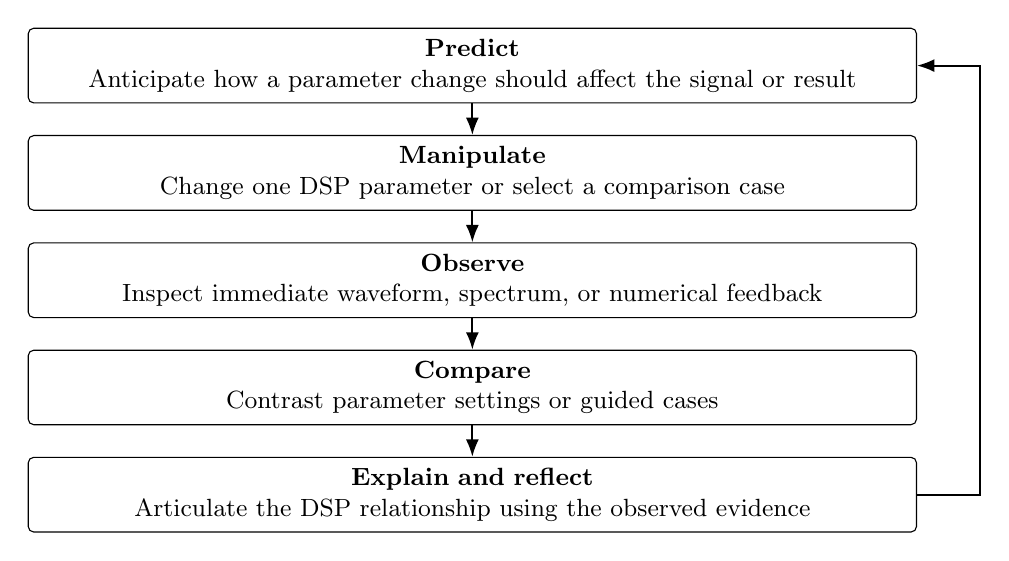
\begin{tikzpicture}[
  font=\small,
  node distance=4mm,
  stage/.style={draw, rounded corners=2pt, align=center, minimum height=8mm, text width=110mm, inner sep=4pt},
  arrow/.style={-{Latex[length=2.2mm]}, line width=0.7pt}
]
\node[stage] (predict) {\textbf{Predict}\\Anticipate how a parameter change should affect the signal or result};
\node[stage, below=of predict] (manipulate) {\textbf{Manipulate}\\Change one DSP parameter or select a comparison case};
\node[stage, below=of manipulate] (observe) {\textbf{Observe}\\Inspect immediate waveform, spectrum, or numerical feedback};
\node[stage, below=of observe] (compare) {\textbf{Compare}\\Contrast parameter settings or guided cases};
\node[stage, below=of compare] (explain) {\textbf{Explain and reflect}\\Articulate the DSP relationship using the observed evidence};

\draw[arrow] (predict) -- (manipulate);
\draw[arrow] (manipulate) -- (observe);
\draw[arrow] (observe) -- (compare);
\draw[arrow] (compare) -- (explain);
\draw[arrow] (explain.east) -- ++(8mm,0) |- (predict.east);
\end{tikzpicture}
\caption{Instructional cycle embedded in the DSP-Lab activities. The design emphasizes guided conceptual comparison rather than unrestricted simulation.}
\label{fig:learning-cycle}
\end{figure}


\section{DSP-Lab Design and Implementation}
\subsection{Application Architecture and Learning Flow}
DSP-Lab is implemented as a native Android application in Kotlin using Jetpack Compose. It is designed to operate offline and does not require a login or cloud backend. This reduces setup burden during ordinary course use and makes the application suitable for short self-directed activities outside class.

The application contains a study entry screen, five DSP learning modules, pre-test and post-test functions, short reflection prompts, and a research-data export function. Learning records are stored locally on the device. The design therefore keeps the technical architecture intentionally simple: the computational and visualization functions are embedded in the app, while research records can be exported as a de-identified CSV file when required.

\subsection{Five Interactive DSP Modules}
Table~\ref{tab:modules} summarizes the five modules. They were selected because each topic contains relationships that can be made more intuitive through direct manipulation and immediate visual feedback.

\begin{table}[htbp]
\centering
\caption{DSP-Lab learning modules and interactive functions.}
\label{tab:modules}
\begin{tabular}{p{0.09\textwidth}p{0.18\textwidth}p{0.28\textwidth}p{0.33\textwidth}}
\toprule
Module & Topic & Conceptual focus & Main interactive function \\
\midrule
01 & Discrete-time signals & Amplitude, frequency, phase, and sequence behavior & Change signal parameters and compare waveform and summary measures \\
02 & Sampling and aliasing & Nyquist condition and aliasing & Change sampling frequency and compare safe, boundary, and aliasing cases \\
03 & Convolution & Shifted overlap and sum of products & Step through convolution and verify selected output samples \\
04 & DFT and spectrum & Bin spacing, alignment, and leakage & Change DFT length and tone frequency and observe spectrum changes \\
05 & FIR filtering & Cutoff and filter-length trade-offs & Change cutoff/tap count and inspect impulse and frequency responses \\
\bottomrule
\end{tabular}
\end{table}

Figure~\ref{fig:app-interface-overview} provides a compact visual overview of the five module interfaces. The panels emphasize the common design pattern rather than Android implementation detail: each screen places a small set of parameters next to an immediately updated DSP representation and a guided comparison or interpretation task.

\begin{figure}[htbp]
\centering
\resizebox{0.98\linewidth}{!}{%
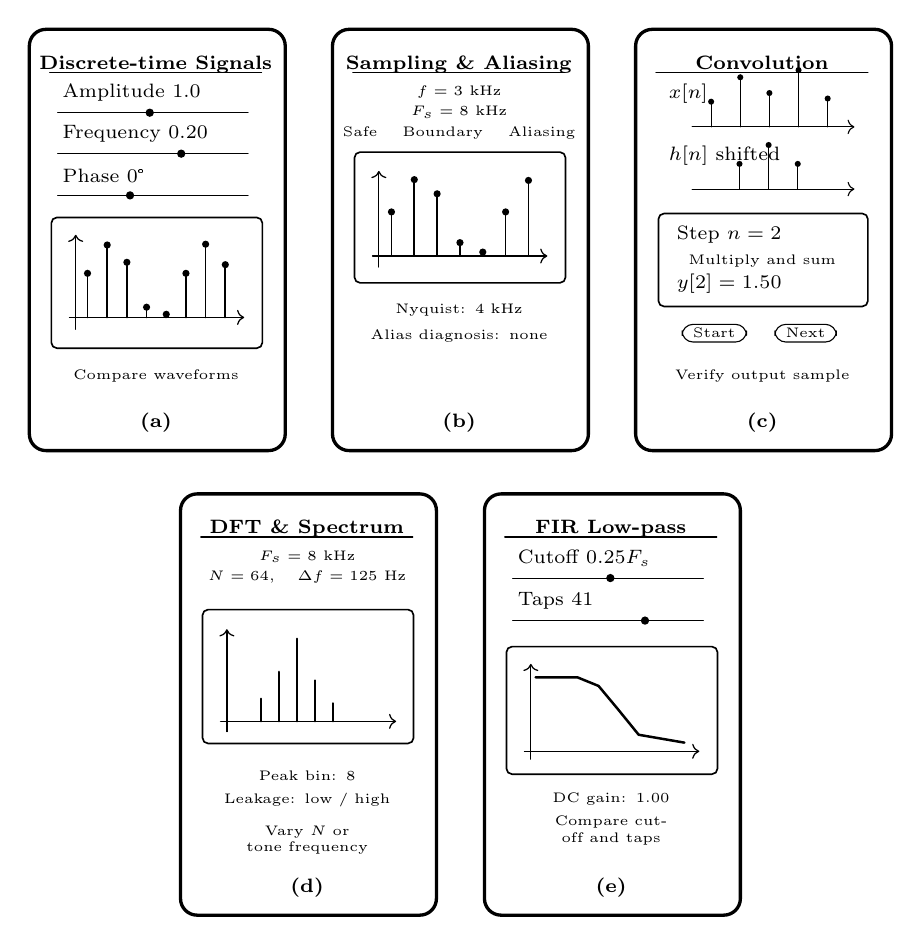
\begin{tikzpicture}[font=\sffamily, line cap=round, line join=round]

\tikzset{
  handset/.style={draw, very thick, rounded corners=6pt, minimum width=3.25cm, minimum height=5.35cm, inner sep=0pt},
  card/.style={draw, rounded corners=2pt, line width=0.6pt},
  tinylabel/.style={font=\scriptsize},
  compactlabel/.style={font=\tiny, align=center, text width=2.45cm},
  paneltitle/.style={font=\bfseries\scriptsize, align=center}
}

% ==================== (a) Signals ====================
\begin{scope}[shift={(0,5.9)}]
  \node[handset, anchor=north west] at (0,0) {};
  \node[paneltitle, anchor=north] at (1.625,-0.23) {Discrete-time Signals};
  \draw[line width=0.5pt] (0.28,-0.57) -- (2.97,-0.57);
  \node[tinylabel, anchor=west] at (0.32,-0.83) {Amplitude  1.0};
  \draw (0.38,-1.08) -- (2.80,-1.08); \fill (1.55,-1.08) circle (1.5pt);
  \node[tinylabel, anchor=west] at (0.32,-1.35) {Frequency  0.20};
  \draw (0.38,-1.60) -- (2.80,-1.60); \fill (1.95,-1.60) circle (1.5pt);
  \node[tinylabel, anchor=west] at (0.32,-1.88) {Phase  0\textdegree};
  \draw (0.38,-2.13) -- (2.80,-2.13); \fill (1.30,-2.13) circle (1.5pt);
  \node[card, minimum width=2.68cm, minimum height=1.66cm, anchor=north west] at (0.29,-2.40) {};
  \draw[->,line width=0.45pt] (0.53,-3.68) -- (2.75,-3.68);
  \draw[->,line width=0.45pt] (0.61,-3.83) -- (0.61,-2.63);
  \foreach \x/\y in {0.76/-3.12,1.01/-2.76,1.26/-2.98,1.51/-3.55,1.76/-3.64,2.01/-3.12,2.26/-2.75,2.51/-3.01} {
    \draw[line width=0.6pt] (\x,-3.68) -- (\x,\y); \fill (\x,\y) circle (1.3pt);
  }
  \node[compactlabel] at (1.63,-4.42) {Compare waveforms};
  \node[font=\bfseries\scriptsize] at (1.63,-5.02) {(a)};
\end{scope}

% ==================== (b) Sampling ====================
\begin{scope}[shift={(3.85,5.9)}]
  \node[handset, anchor=north west] at (0,0) {};
  \node[paneltitle, anchor=north] at (1.625,-0.23) {Sampling \& Aliasing};
  \draw[line width=0.5pt] (0.28,-0.57) -- (2.97,-0.57);
  \node[font=\tiny, align=center] at (1.63,-0.82) {$f=3$ kHz};
  \node[font=\tiny, align=center] at (1.63,-1.07) {$F_s=8$ kHz};
  \node[font=\tiny, align=center] at (1.63,-1.34) {Safe \quad Boundary \quad Aliasing};
  \node[card, minimum width=2.68cm, minimum height=1.66cm, anchor=north west] at (0.29,-1.57) {};
  \draw[->,line width=0.45pt] (0.53,-2.90) -- (2.75,-2.90);
  \draw[->,line width=0.45pt] (0.61,-3.04) -- (0.61,-1.82);
  \foreach \x/\y in {0.77/-2.34,1.06/-1.93,1.35/-2.11,1.64/-2.73,1.93/-2.85,2.22/-2.34,2.51/-1.94} {
    \draw[line width=0.6pt] (\x,-2.90) -- (\x,\y); \fill (\x,\y) circle (1.3pt);
  }
  \node[compactlabel] at (1.63,-3.59) {Nyquist: 4 kHz};
  \node[compactlabel] at (1.63,-3.91) {Alias diagnosis: none};
  \node[font=\bfseries\scriptsize] at (1.63,-5.02) {(b)};
\end{scope}

% ==================== (c) Convolution ====================
\begin{scope}[shift={(7.70,5.9)}]
  \node[handset, anchor=north west] at (0,0) {};
  \node[paneltitle, anchor=north] at (1.625,-0.23) {Convolution};
  \draw[line width=0.5pt] (0.28,-0.57) -- (2.97,-0.57);
  \node[tinylabel, anchor=west] at (0.32,-0.84) {$x[n]$};
  \draw[->,line width=0.4pt] (0.74,-1.26) -- (2.80,-1.26);
  \foreach \x/\h in {0.98/0.32,1.35/0.63,1.72/0.43,2.09/0.72,2.46/0.36}{\draw (\x,-1.26)--(\x,{-1.26+\h});\fill (\x,{-1.26+\h}) circle (1.1pt);}
  \node[tinylabel, anchor=west] at (0.32,-1.63) {$h[n]$ shifted};
  \draw[->,line width=0.4pt] (0.74,-2.05) -- (2.80,-2.05);
  \foreach \x/\h in {1.34/0.32,1.71/0.56,2.08/0.32}{\draw (\x,-2.05)--(\x,{-2.05+\h});\fill (\x,{-2.05+\h}) circle (1.1pt);}
  \node[card, minimum width=2.66cm, minimum height=1.18cm, anchor=north west] at (0.30,-2.35) {};
  \node[tinylabel, anchor=west] at (0.42,-2.63) {Step $n=2$};
  \node[compactlabel] at (1.63,-2.96) {Multiply and sum};
  \node[tinylabel, anchor=west] at (0.42,-3.25) {$y[2]=1.50$};
  \node[font=\tiny, draw, rounded corners=4pt, inner xsep=4pt, inner ysep=1.5pt] at (1.02,-3.88) {Start};
  \node[font=\tiny, draw, rounded corners=4pt, inner xsep=4pt, inner ysep=1.5pt] at (2.18,-3.88) {Next};
  \node[compactlabel] at (1.63,-4.42) {Verify output sample};
  \node[font=\bfseries\scriptsize] at (1.63,-5.02) {(c)};
\end{scope}

% ==================== (d) DFT ====================
\begin{scope}[shift={(1.92,0)}]
  \node[handset, anchor=north west] at (0,0) {};
  \node[paneltitle, anchor=north] at (1.625,-0.23) {DFT \& Spectrum};
  \draw[line width=0.5pt] (0.28,-0.57) -- (2.97,-0.57);
  \node[font=\tiny, align=center] at (1.63,-0.82) {$F_s=8$ kHz};
  \node[font=\tiny, align=center] at (1.63,-1.08) {$N=64,\quad \Delta f=125$ Hz};
  \node[card, minimum width=2.68cm, minimum height=1.70cm, anchor=north west] at (0.29,-1.48) {};
  \draw[->,line width=0.45pt] (0.53,-2.91) -- (2.76,-2.91);
  \draw[->,line width=0.45pt] (0.61,-3.04) -- (0.61,-1.74);
  \draw[line width=0.75pt] (1.04,-2.91)--(1.04,-2.62);
  \draw[line width=0.75pt] (1.27,-2.91)--(1.27,-2.28);
  \draw[line width=0.75pt] (1.50,-2.91)--(1.50,-1.86);
  \draw[line width=0.75pt] (1.73,-2.91)--(1.73,-2.39);
  \draw[line width=0.75pt] (1.96,-2.91)--(1.96,-2.68);
  \node[compactlabel] at (1.63,-3.60) {Peak bin: 8};
  \node[compactlabel] at (1.63,-3.91) {Leakage: low / high};
  \node[compactlabel] at (1.63,-4.42) {Vary $N$ or tone frequency};
  \node[font=\bfseries\scriptsize] at (1.63,-5.02) {(d)};
\end{scope}

% ==================== (e) FIR ====================
\begin{scope}[shift={(5.78,0)}]
  \node[handset, anchor=north west] at (0,0) {};
  \node[paneltitle, anchor=north] at (1.625,-0.23) {FIR Low-pass};
  \draw[line width=0.5pt] (0.28,-0.57) -- (2.97,-0.57);
  \node[tinylabel, anchor=west] at (0.32,-0.84) {Cutoff  $0.25F_s$};
  \draw (0.38,-1.09) -- (2.80,-1.09); \fill (1.62,-1.09) circle (1.5pt);
  \node[tinylabel, anchor=west] at (0.32,-1.38) {Taps  41};
  \draw (0.38,-1.63) -- (2.80,-1.63); \fill (2.06,-1.63) circle (1.5pt);
  \node[card, minimum width=2.68cm, minimum height=1.62cm, anchor=north west] at (0.29,-1.95) {};
  \draw[->,line width=0.45pt] (0.53,-3.29) -- (2.75,-3.29);
  \draw[->,line width=0.45pt] (0.61,-3.39) -- (0.61,-2.18);
  \draw[line width=0.9pt] (0.67,-2.35) -- (1.20,-2.35) -- (1.47,-2.46) -- (1.72,-2.76) -- (1.98,-3.08) -- (2.56,-3.18);
  \node[compactlabel] at (1.63,-3.90) {DC gain: 1.00};
  \node[compactlabel] at (1.63,-4.30) {Compare cutoff and taps};
  \node[font=\bfseries\scriptsize] at (1.63,-5.02) {(e)};
\end{scope}

\end{tikzpicture}%
}
\caption{Representative DSP-Lab interface overview. The schematic panels summarize the common mobile interaction pattern across the five learning modules: parameter adjustment, immediate graphical or numerical feedback, guided comparison, and short explanation. (a) discrete-time signals; (b) sampling and aliasing; (c) convolution; (d) DFT and spectrum; and (e) FIR filtering.}
\label{fig:app-interface-overview}
\end{figure}


In the sampling module, the learner can compare the signal frequency with the sampling frequency and directly observe whether a case is safely sampled or aliased. In the DFT module, the relationship
\begin{equation}
\Delta f = \frac{F_s}{N}
\end{equation}
is linked to the displayed spectrum so that changes in $N$ can be inspected immediately. In the convolution module, students can inspect the stepwise multiply-and-sum process rather than treating convolution only as a final numerical result. In the FIR module, increasing filter length or changing cutoff frequency produces an immediate response change, allowing students to compare design trade-offs without first writing a complete filter-design program.

\subsection{Guided Interaction and Reflection}
The five modules use the same learning logic even though the DSP calculations differ. Students are first asked to anticipate a result, then modify one or more parameters, inspect the resulting visualization or numerical output, compare selected cases, and finally write a short explanation. The aim is to make exploration structured rather than completely open-ended.

This interaction pattern is especially suitable for after-class review because the activity can remain short. A typical module is intended to require approximately 15--30 minutes. The application is therefore positioned between static review materials and more comprehensive MATLAB/Python laboratory work.

\subsection{Learning Records and Research Support}
For teaching evaluation, DSP-Lab records module completion, final parameter values, elapsed activity duration, reflection text, and submission time. The recorded duration is treated only as an approximate engagement indicator because elapsed screen time is not identical to continuous cognitive engagement. The research dashboard also supports an anonymous participant code and CSV export so that classroom data can be analyzed without requiring a network service.

\section{Teaching Evaluation}
\subsection{Participants and Procedure}
The evaluation uses a simple pre-test/post-test comparison in an undergraduate DSP course at \tbd{anonymous institution}. The study includes \tbd{experimental n} students using DSP-Lab and \tbd{control n} students completing conventional topic-matched review. Both groups follow the same core course content and complete the same five topic areas over approximately five instructional weeks.

Before the intervention, both groups complete a 12-item Form A concept test. During the five-week period, the experimental group completes the corresponding DSP-Lab activity after each topic, whereas the comparison group completes conventional review material covering the same topic. After the intervention, both groups complete a parallel 12-item Form B concept test. Students in the DSP-Lab group additionally complete a short 10-item five-point questionnaire on usefulness, visualization, interaction, ease of use, self-directed learning support, and willingness to use similar activities.

The concept tests cover discrete-time signals (2 items), sampling and aliasing (3 items), convolution (2 items), DFT/spectrum (3 items), and FIR filtering (2 items). The items were reviewed by \tbd{number} instructors with DSP teaching experience before classroom use. The study was conducted under the participating institution's applicable ethics/consent requirements. \tbd{Insert approval/exemption and consent statement.}

% Publication-ready vector figure: quasi-experimental study flow
\begin{figure}[htbp]
\centering
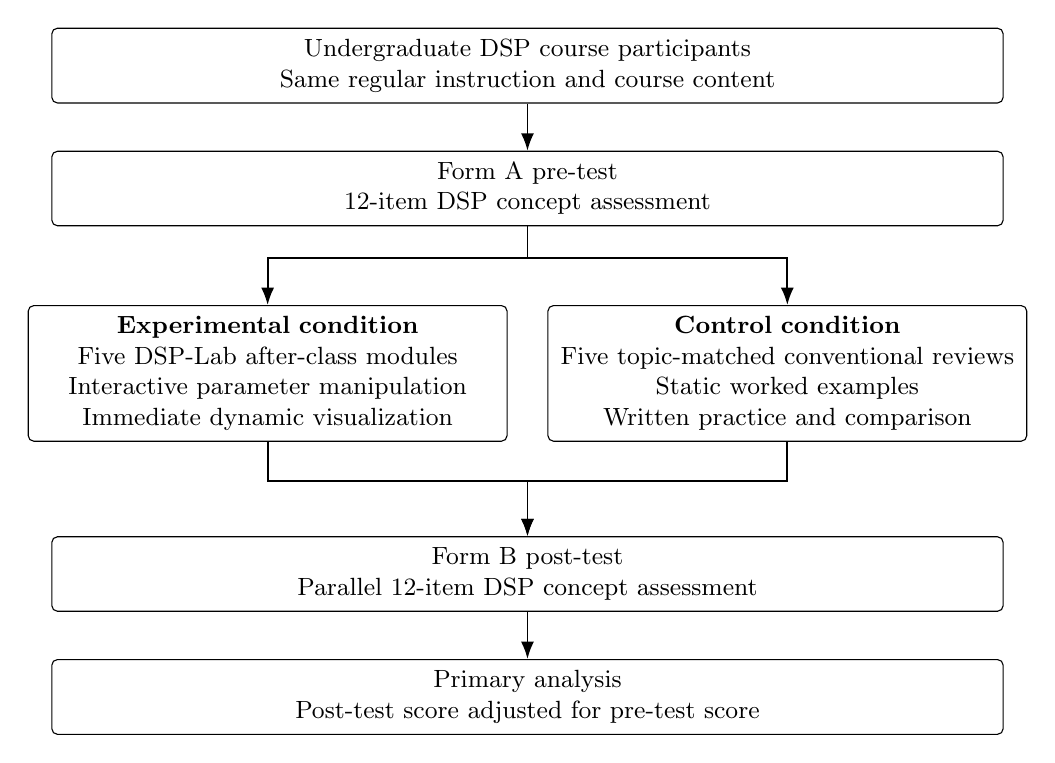
\begin{tikzpicture}[
  font=\small,
  node distance=6mm,
  box/.style={draw, rounded corners=2pt, align=center, minimum height=8mm, text width=118mm, inner sep=4pt},
  branch/.style={draw, rounded corners=2pt, align=center, minimum height=16mm, text width=58mm, inner sep=4pt},
  arrow/.style={-{Latex[length=2.2mm]}, line width=0.7pt}
]

\node[box] (participants) {Undergraduate DSP course participants\\Same regular instruction and course content};
\node[box, below=of participants] (pre) {Form A pre-test\\12-item DSP concept assessment};

\node[branch, below=10mm of pre, xshift=-33mm] (exp) {\textbf{Experimental condition}\\Five DSP-Lab after-class modules\\Interactive parameter manipulation\\Immediate dynamic visualization};
\node[branch, below=10mm of pre, xshift=33mm] (ctl) {\textbf{Control condition}\\Five topic-matched conventional reviews\\Static worked examples\\Written practice and comparison};

\coordinate (branchmid) at ($(exp.south)!0.5!(ctl.south)$);
\node[box, below=12mm of branchmid] (post) {Form B post-test\\Parallel 12-item DSP concept assessment};
\node[box, below=of post] (analysis) {Primary analysis\\Post-test score adjusted for pre-test score};

\draw[arrow] (participants) -- (pre);
\draw[arrow] (pre.south) -- ++(0,-4mm) -| (exp.north);
\draw[arrow] (pre.south) -- ++(0,-4mm) -| (ctl.north);
\draw[arrow] (exp.south) -- ++(0,-5mm) -| (post.north);
\draw[arrow] (ctl.south) -- ++(0,-5mm) -| (post.north);
\draw[arrow] (post) -- (analysis);

\end{tikzpicture}
\caption{Quasi-experimental study flow. Both groups receive the same regular DSP instruction; the planned contrast is the form of after-class learning support.}
\label{fig:study-flow}
\end{figure}


\subsection{Data Analysis}
The analysis is intentionally limited. Pre-test and post-test scores are summarized using means and standard deviations. The main comparison uses post-test score as the outcome while adjusting for pre-test score:
\begin{equation}
\mathrm{PostScore}_i = \beta_0 + \beta_1\mathrm{Group}_i + \beta_2\mathrm{PreScore}_i + \varepsilon_i.
\end{equation}
The adjusted group difference is reported with a 95\% confidence interval and $p$ value. For scale interpretation, the unadjusted post-test Experimental-minus-Control Cohen's $d$ is reported separately as a descriptive standardized difference rather than as an adjusted ANCOVA effect size. Within-group pre/post change and raw gain are supporting results. Questionnaire items are summarized descriptively using means and standard deviations; they are interpreted as student perceptions rather than as direct evidence of learning effectiveness.

\section{Results and Discussion}
\subsection{Learning Outcomes}
Table~\ref{tab:outcomes} is intentionally compact so that the primary outcome can be read without a large statistical table.

\begin{table}[htbp]
\centering
\caption{Learning outcomes by group. Replace dashes after data collection.}
\label{tab:outcomes}
\small
\begin{tabular}{lcccc}
\toprule
Group & $n$ & Pre-test M (SD) & Post-test M (SD) & Raw gain M (SD) \\
\midrule
DSP-Lab & -- & -- & -- & -- \\
Control & -- & -- & -- & -- \\
\bottomrule
\end{tabular}
\end{table}

\tbd{Primary result: After adjustment for pre-test score, report the DSP-Lab-minus-Control post-test difference in score points, 95\% CI, and p value. Then report the unadjusted post-test Cohen's d as a descriptive standardized difference.}

\tbd{Secondary result: Report the DSP-Lab group's pre-test mean, post-test mean, mean change, paired p value, and paired Cohen's d in one sentence.}

The primary interpretation should be based on the adjusted between-group estimate and its confidence interval rather than on statistical significance alone. If the estimate favors DSP-Lab, the result is consistent with the possibility that direct parameter manipulation and immediate visual feedback helped students connect abstract DSP relationships with observable consequences. This mechanism should remain an instructional interpretation rather than a separate causal claim because the individual design components were not experimentally isolated.

\subsection{Student Experience}
The questionnaire is used only as a secondary measure of student experience. A short summary is sufficient for the main paper; a full 10-item table can be moved to supplementary material if requested.

\begin{table}[htbp]
\centering
\caption{Compact summary of DSP-Lab student experience.}
\label{tab:questionnaire-summary}
\begin{tabular}{p{0.58\textwidth}p{0.28\textwidth}}
\toprule
Measure & Observed result \\
\midrule
Questionnaire participants & -- \\
Overall 10-item mean (SD) & -- \\
Cronbach's $\alpha$ & -- \\
Highest-rated item, mean (SD) & -- \\
Lowest-rated item, mean (SD) & -- \\
\bottomrule
\end{tabular}
\end{table}

\tbd{Report the overall questionnaire mean, internal consistency, and the highest- and lowest-rated items with their means/SDs. Keep the paragraph descriptive and concise.}

Questionnaire findings should complement the objective learning outcome. High ratings for visualization, interaction, or mobile convenience can support claims about perceived usefulness and usability, but they should not be presented as proof of learning effectiveness by themselves.

\subsection{Educational Implications and Limitations}
DSP-Lab is intended as a supplementary learning tool rather than a replacement for conventional DSP lectures, programming assignments, or hardware laboratories. Its practical value lies in allowing students to test conceptual relationships quickly on a mobile device before or after more comprehensive laboratory work. This complementary role is consistent with engineering-education literature that treats virtual and interactive tools as additions to, rather than automatic substitutes for, conventional learning experiences \citep{li2024}.

The evaluation is deliberately modest. Its main limitations are expected to include the use of a single course or institution, a relatively short intervention period, researcher-developed concept tests and questionnaire, and possible differences between intact student groups if class-level assignment is used. These limitations should be stated directly, and the results should be interpreted as classroom evidence of educational usefulness rather than definitive causal proof across institutions.

\section{Conclusion}
This paper presents DSP-Lab, a compact Android application that supports undergraduate DSP learning through direct parameter manipulation, immediate visualization, guided comparison, and short reflection across five core topics. The application was designed for short after-class use and to complement, rather than replace, conventional lectures and programming laboratories. \tbd{Insert one sentence for the adjusted learning result and one sentence for the student-experience result.} The combined application design and classroom evaluation provide a practical example of how mobile interaction can be integrated into undergraduate DSP education without requiring a complex learning platform or large-scale experimental study.

\section*{Data Availability Statement}
\tbd{State whether de-identified data and analysis code can be shared publicly, on reasonable request, or under ethics/privacy restrictions.}

\section*{Conflict of Interest}
The authors declare no conflict of interest.

\bibliographystyle{unsrtnat}
\bibliography{references}

\end{document}
